\chapter{Path Indexing}
In this section an informal overview of path indexing is given. Both the theoretical concept and some details of its implementation in Isabelle/ML are discussed.\\
Path indexing is based on mapping each symbol of a term to a path. This path consists of the nodes traversed from the root to the symbol. In the standard tree form this is an alternating sequence of symbols and the index of the argument which is traversed next.\\
\begin{figure}[h]
\centering
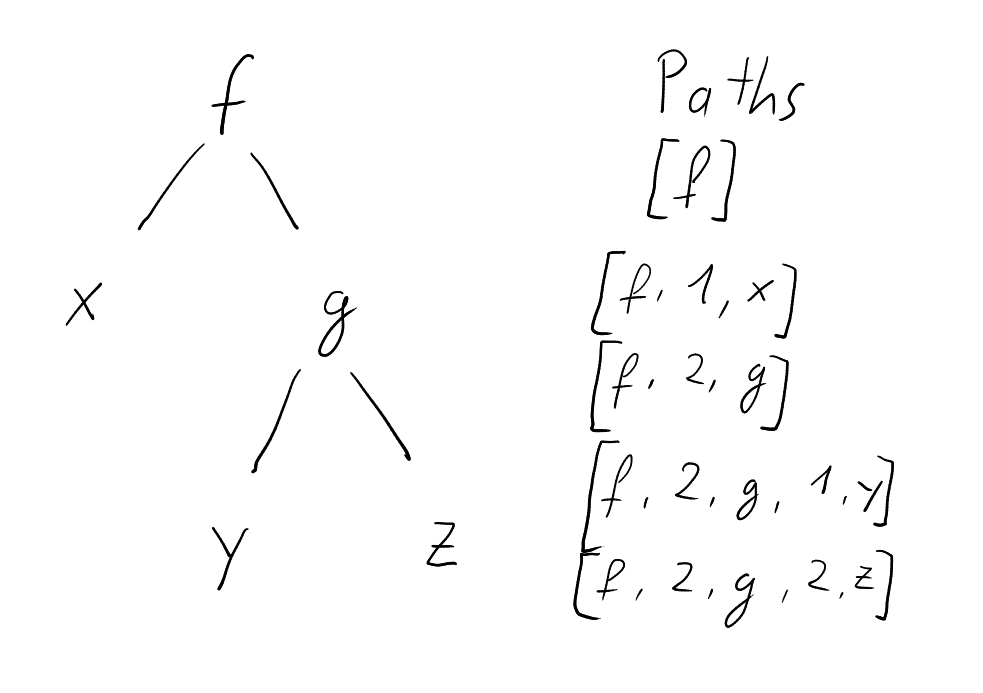
\includegraphics[scale=0.25]{figures/term_path.png}
\caption{A term and the paths associated with its symbols}
\end{figure}\\
The term index itself consists of a collection of paths with each path storing a list of terms that contain a symbol with this path. Consequently each term is stored at as many locations as it has symbols.\\
A query for variants of a term is resolved by collecting the path lists associated with each symbol. These path lists are then intersected to retain only those terms that have identical symbols at all positions. More complex queries like instances, generalisations and unifiables are handled by introducing unions of two recursive calls or ignoring variables.\\
The queries are not exact and may return extra terms. For example an index containing both ``f x'' and ``f x y'' will return both terms when queries for variants of ``f x''. This is consequence of the fact that the total number of arguments of a function is not stored and ``f x y'' matches ``f x'' on all its symbols. Additionally the name of variables is not stored as all queries except the lookup handle them indifferently which reduces the number of unions required.\\
